\documentclass{beamer}


\usepackage{amsmath}
\usepackage[style=alphabetic,url=true]{biblatex}
\usepackage{environ}
\usepackage{geometry}
\usepackage{graphicx}
\usepackage{tikz}
\usepackage[T2A]{fontenc}
\usepackage[utf8]{inputenc}
\usepackage{listings}
\usepackage{cancel}
\usepackage{soul}


% \usetheme{Bergen}

\usecolortheme{beaver}

\setbeamertemplate{itemize item}[circle]
\setbeamertemplate{itemize subitem}{--}
\addtobeamertemplate{navigation symbols}{}{
  \usebeamerfont{footline}%
  \usebeamercolor[fg]{footline}%
  \hspace{1em}%
  \insertframenumber/\inserttotalframenumber
}
\graphicspath{ {./graphics/} }


\title{
  Біткоїн та криптовалютні технології \\
  Лекція 1: Економіка та історія
}

\author{Юрій Жикін}
\date{17 лютого, 2025}

\begin{document}

\frame{\titlepage}

\begin{frame}
  \frametitle{Економічні концепції та властивості грошей}
  \begin{itemize}
  \item \textbf{Гроші - це будь які об'єкти, що широко приймаються як плата за
      товари та послуги}
  \item \textbf{Стійкість} - гроші повинні зберігати свою цінність з плином часу
  \item \textbf{Портативність} - гроші повинні бути легкими для транспортування
    у відносно великих кількостях
  \item \textbf{Подільність} - гроші повинні ділитись на дрібні ``шматки'' для
    представлення всього діапазону вартості
  \item \textbf{Взаємозамінність} - дві грошові одиниці тієї ж номінальної
    вартості повинні бути однаково цінними
  \item \textbf{Дефіцитність} - складно збільшити пропозицію грошей на ринку
  \item \textbf{Впізнаваність} - легко знайти учасників ринку, які готові
    прийняти дану грошову одиницю як плату за товари чи послуги
  \end{itemize}
\end{frame}

\begin{frame}
  \frametitle{Гроші до Біткоїна}
  \begin{itemize}
  \item Мушлі
  \item Срібло
  \item Золото
  \item Паперові гроші
  \item Декретні (указові, або фіатні) гроші
  \end{itemize}
\end{frame}

\begin{frame}
  \frametitle{Централізовані електронні гроші 1/2}
  \begin{itemize}
  \item Традиційні електронні гроші - централізовані ``бухгалтерські книги''
    (банківські бази даних)
    \begin{itemize}
    \item рахунок: ``хто, скільки''
    \item переказ: ``хто, скільки, кому''
    \end{itemize}
  \item Транзакції в межах одного банку змінюють значення ``баланс рахунку''
    адресата та адресанта транзакції
  \item Транзакції між банками - перекази між банками, що агрегують платежі між
    клієнтами різних банків (SWIFT)
  \end{itemize}
  
\end{frame}

\begin{frame}
  \frametitle{Централізовані електронні гроші 2/2}
  \begin{itemize}
  \item В більшості випадків держава є сутністю, яка централізовано контролює
    пропозицію грошей на ринку
  \item Чи є ``держава'' достатньо компетентною для того, щоб ``керувати''
    економікою, в якій беруть участь мільйони учасників?
  \item Державний апарат може довільно збільшувати пропозицію фіатних грошей на
    ринку, фактично ``витягуючи'' ресурси у \textbf{всіх} своїх громадян без
    їхнього дозволу через зменшення купівельної спроможності їхніх заощаджень
  \item Повний контроль над грошовою системою є основним інструментом контролю
    над людьми в тоталітарних режимах
  \end{itemize}
\end{frame}

\begin{frame}
  \frametitle{Децентралізовані електронні гроші}
  \begin{itemize}
  \item \textbf{Економічний анархізм}: держава не повинна втручатись в приватну
    економічну діяльність індивідуумів.
  \item Чи можливо усунути централізоване управління електронними грошима?
  \item \textbf{Проблема візантійських генералів} - як можуть декілька генералів
    домовитись про наступ, якщо вони не довіряють один одному?
  \item \textbf{Як можуть декілька учасників ринку досягнути консенсусу без
      необхідності довіряти один одному?}
  \end{itemize}
\end{frame}

\begin{frame}
  \frametitle{Криптографія і шифропанк-рух}
  \begin{itemize}
  \item \textbf{Криптографія} - це сукупність методів захисту інформації і
    комунікації від зовнішнього впливу
  \item ``Широке використання сильної криптографії і технологій посилення
    приватності персональних даних - це шлях до соціальних та політичних змін на
    краще''
  \item \textbf{Чи можемо ми використовувати сильну криптографію для того, щоб
      вирішити задачу візантійських генералів і створити де централізовану
      грошову систему?}
  \item Декілька спроб:
    \begin{itemize}
    \item Девід Чом (David Chaum) - DigiCash, 1989
    \item Вей Дай (Wei Dai) - b-money, 1998
    \item Нік Забо (Nick Szabo) - Bit Gold, 1998
    \item Адам Бек (Adam Back) - Hashcash, 1997-2002
    \end{itemize}
  \end{itemize}
\end{frame}

\begin{frame}
  \frametitle{Сатоші Накамото та створення Біткоїна 1/3}
  \begin{itemize}
  \item Фінансова криза 2007-2008 років
  \item 31 жовтня 2008 року особа під псевдонімом \textbf{Сатоші Накамото}
    опублікувала статтю під назвою ``Біткоїн: однорангова система електронної готівки''
  \item В кінці 2008 - на початку 2009 років, Накамото почав спілкуватись з Вей
    Дай, Адамом Беком та Халом Фінні щодо електронної готівкової системи, над
    якою він працював
  \item 3 січня 2009 року, Накамото випустив версію 0.1 програмного забезпечення
    Біткоїн і запустив мережу, змайнивши перший блок (\textbf{генезисний блок})
  \end{itemize}
\end{frame}

\begin{frame}[fragile]
  \frametitle{Сатоші Накамото і створення Біткоїна 2/3}
  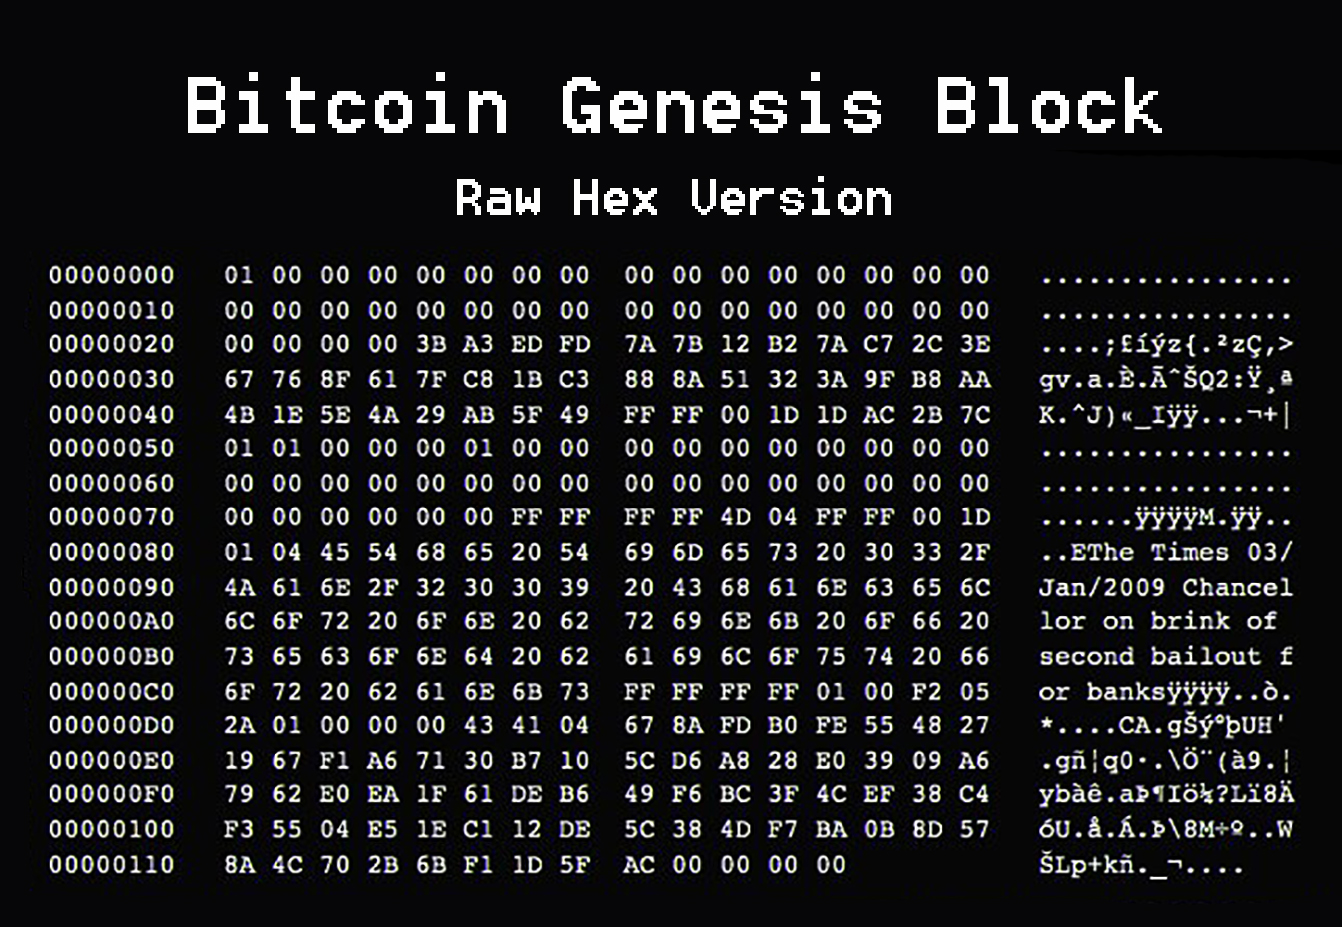
\includegraphics[width=\textwidth]{genesis-block}
\end{frame}

\begin{frame}
  \frametitle{Сатоші Накамото і створення Біткоїна 3/3}
  \begin{itemize}
  \item Сатоші Накамото продовжує працювати на Біткоїном до середини 2010 року,
    коли він передає контроль над репозиторієм з кодом програмного забезпечення
    Гейвіну Андерсену
  \item 26 квітня 2011 року Накамото пише свій останній відомий лист Андерсену,
    після чого більше ніколи не з'являється у мережі
  \item Програмне забезпечення, написане Сатоші Накамото, перетворилось у проект
    під назвою ``Біткоїн-ядро'' (Bitcoin Core project - https://github.com/bitcoin/bitcoin)
  \end{itemize}
\end{frame}

\begin{frame}
  \frametitle{Новизна Біткоїна}
  \begin{itemize}
  \item Криптографічний алгоритм ``доказу виконаної роботи'' є першим в історії
    повноцінним вирішенням загальної проблеми візантійських генералів, що усуває
    необхідність довіри між учасниками мережі для досягнення консенсусу
  \item \textbf{Біткоїн - повністю децентралізована грошова система}
  \item Система тразнакційних скриптів робить Біткоїн-протокол надзвичайно
    гнучким та придатним для багатьох інших функцій, окрім простої передачі
    цінності
  \item \textbf{Біткоїн - це гроші, які можна програмувати}
  \end{itemize}
\end{frame}

\begin{frame}
  \frametitle{Визнання ринком 1/2}
  \begin{itemize}
  \item В 2010 році була здіснена перша відома комерційна транзакція з
    використання біткоїна - програміст Лазло Ханьєч придбав дві піци Papa John's
    за 10000 біткоїнів
  \item В 2011 році біткоїн починає прийматись як благодійні внески
    організаціями Electronic Frontier Foundation та WikiLeaks
  \item У 2011 році ціна зросла з \$0.30 до \$5.27
  \item У 2012 році - з \$5.25 до \$13.30
  \item У 2013 році - з \$13.30 до \$770
  \item У жовтні 2021 року ціна біткоїна сягнула \$65000.00
  \end{itemize}
\end{frame}

\begin{frame}[fragile]
  \frametitle{Визнання ринком 2/2}
  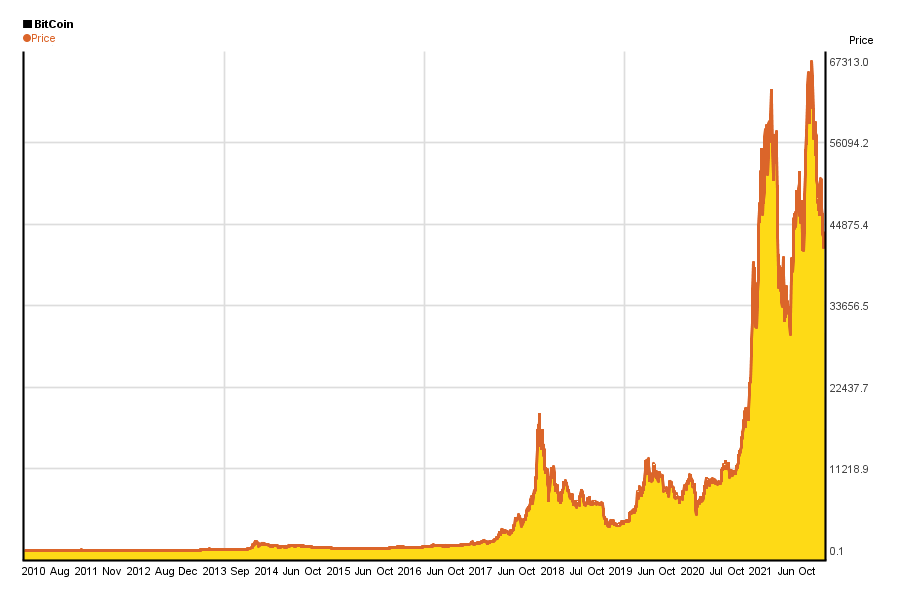
\includegraphics[width=\textwidth]{bitcoin-price}
\end{frame}

\begin{frame}
  \frametitle{Додаткові ресурси}
  \begin{itemize}
  \item https://www.activism.net/cypherpunk/manifesto.html - Cypherpunk Manifesto
  \item https://unenumerated.blogspot.com - Nick Szabo's Blog
  \item The Bitcoin Standard: The Decentralized Alternative to Central Banking,
    2018 - Saifedean Ammous
  \item Human Action: A Treatise on Economics, 1949 - Ludwig von Mises
  \end{itemize}
\end{frame}

\begin{frame}
  \frametitle{Кінець}
  \begin{center}
    Дякую за увагу!
  \end{center}
\end{frame}

\end{document}

%%% Local Variables:
%%% mode: latex
%%% TeX-master: t
%%% End:
